%!TEX root = main.tex

\section{Analysis of Video Frames}
\label{sec:frame-analysis}

As mentioned in Section~\ref{sec:system}, different frames in H.264 have different frame size and production speed, which may result in different network performance. In this section we will analyze in detail the different performance of I,P and V frame in TCP download flows. 

\subsection{Base video frame information}
\label{sub:base-frame}

Table~\ref{tab:frames-info} shows the statistics of different frames. Among all the three frames, P frame takes up 82.8 \% of all frames and is the largest part of all frames. The V frame has the smallest percentage of all frames just 5.8\% and that of I frame is 11.5\%. In this system the production intervals of I and V frames are set to 4s and 0.04s respectively. For download flows, the interval begins as the server sends out a frame till it sends out next frame with the same type. We find the actual intervals of I and V frames are 4.85s and 0.069s respectively because RTT jitter and packet loss may delay the frames. P frame has production interval 0.081s. I frame is the largest frame whose average size is 30 Kbytes. P frame's average size is 3.4 Kbytes while the V frame is just 189 bytes, much smaller than the other two. The different frame size results in different burst packet number for different frames. V frame has no burst packet as its size is less than one packet size(most of the packet size is around 1460 bytes, the same with MTU). The number of burst packets of about 15\% P frames is larger than 5 packets, while 40\% of I frames are more than 5 burst packets. Routers are likely to drop burst packets, so the I frame's packet loss rate is 1.1\% which is higher than other two frames. P and I frame's packet loss rate is 0.6\% and 0.61\% respectively. Among these lost packets, some result in timeout retransmissions, as they can not be recovered by fast retransmit. For I frame, 11.8\% of loss packets result in timeout retransmissions while for P frame and V frame the ratios are 11.3\% and 14\% respectively. In Section~\ref{sub:timeout-frame} we will detail the timeout retransmissions of different frames.

\begin{table}
\tablefontsize
\renewcommand{\arraystretch}{\assize}
\setlength{\tabcolsep}{3pt}
\caption{Analysis for different frames.}
%\label{tab:analysis-frames}
\centering
\subtable[Base information of different frame.]{
\begin{tabular}{c|c|c|c|c|c}
	\toprule
	type  & per(\%) & interval(s) & size(B) &  loss rate(\%) &  timeout/loss(\%) \\
	\hline
	I   & 11.5 & 4.85 & 30K & 1.1  & 11.8 \\
	\hline
	P  & 82.8 & 0.081 & 3.4K  & 0.6 & 11.3 \\
	\hline
	V   & 5.8 & 0.069 & 189 & 0.61  & 14 \\
	\bottomrule
\end{tabular}
\label{tab:frames-info}
}

\subtable[Ratio of timeout retransmissions for different frames.]{
\centering
\begin{tabular}{c|c|c|c}
	\toprule
	timeout retrans. type & I frame(\%) & P frame(\%) & V frame(\%)\\
	\hline
	tail retrans. & 3.8 & 4.0 & 5.0 \\
	\hline
	less pkt retrans. & 11.4 & 20.2 & 30.8 \\
	\hline
	double retrans. & 46.8 & 44.7 & 47.2 \\
	\hline
	ACK delay/loss & 19.1 & 15.1 & 8.5 \\
	\hline
	continuous loss & 4.2 & 1.5 & 0 \\
	\hline
	others & 14.7 & 14.4 & 8.5 \\
	\bottomrule
\end{tabular}
\label{tab:time-out-frames}
}
\end{table}

\iffalse
\begin{figure}[ht]
	\centering
	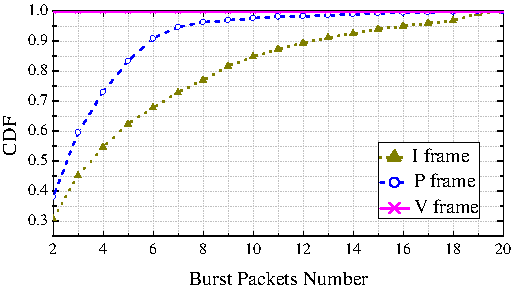
\includegraphics[width=\linewidth]{burst-frame}
	\caption{Different number of burst packets for different frames.}
	\label{fig:burst-frame}
	\termspace
\end{figure}
\fi

\subsection{Timeout retransmission of video frames}
\label{sub:timeout-frame}

If fast retransmit fails to be triggered to recover packet loss, sender has to rely on costly timeout retransmission~\cite{flach2013reducing}. According the situation when the timeout retransmission happens, the timeout retransmission can be divided into several types. If the retransmitted packet by fast retransmit is dropped by the network, timeout retransmission has to be triggered and we refer this timeout retransmission as \emph{double retrans}. If the lost packet is in the last three packets of the frame, there are not enough duplicate acknowledgments (dupacks) to trigger fast retransmit, we refer it as \emph{tail retransmission}. Insufficient number of dupacks to trigger fast retransmit may also due to that the server sends less than 4 packets out(limited by either cwnd or rwnd), and we refer it as \emph{less pkt retransmission}. The ACK delay/loss or all packets sent out lost will also result in timeout retransmission, as at both of the two situations no dupacks can be produced. We refer the two timeout retransmissions as \emph{ACK delay/loss} and \emph{continuous loss} respectively. 

Table~\ref{tab:time-out-frames} shows the ratio of each type of timeout retransmission for I, P and V frame. Those that cannot be classified into any of the above types are referred to as \emph{others}. For all of the frames, double retrans contributes the largest part of the timeout retransmissions, 46.8\% for I frame, 44.7\% for P frame and 47.2\% for V frame. That is because when the network drops a packet, the network has a high probability to become congested so the retransmitted packet via fast retransmit is likely to be dropped again. For V frame, the ratio of less pkt retransmission is 30.8\%, much higher than that for I and P frame (11.4\% and 20.2\% respectively). As the V frame is less than one MSS, when sending the V frame, there are often few packets in the network compared with that when sending I frame. This explains not only the higher ratio of less pkt retransmission for V frame, but also the higher ratio of timeout retransmission for V frame despite the lower packet loss rate (shown in Table~\ref{tab:frames-info}). The I and P frames contain larger number of burst packets, the time that it is stored in the router is longer than that of V frame, so for I and P frames the ratios of ACK delay/loss timeout retransmission are 19.1\% and 15.1\% respectively, much higher than that for V frame. Also because the different number of burst packets, the ratio of continuous loss for V frame is 0, while those for I and P frames are 4.2\% and 1.5\% respectively.

